\documentclass{article}
\usepackage{amsmath}
\usepackage{amsthm}
\usepackage{amsfonts}
\usepackage{mathrsfs}
\usepackage{bm}
\usepackage{listings}
\usepackage[usenames,dvipsnames]{xcolor}
\usepackage{tikz}
\usepackage[margin=1.2in]{geometry}
\usepackage{hyperref}

\hypersetup{
    colorlinks,
    linkcolor={red!30!black},
    citecolor={blue!50!black},
    urlcolor={blue!80!black}
}


\newcommand{\vct}[1]{\mathbf{#1}}
\newcommand{\vx}{\vct{x}}
\newcommand{\vy}{\vct{y}}
\newcommand{\Z}{\mathcal{Z}}
\newcommand{\E}{\mathcal{E}}
\newcommand{\Ham}{\mathcal{H}}
\newcommand{\W}{\mathcal{W}}
\newcommand{\A}{\mathcal{A}}
\newcommand{\LL}{\mathcal{L}}
\newcommand{\var}{\mathrm{var}}
\newcommand{\com}{\mathrm{com}}

\newcommand{\llbra}{[\![}
\newcommand{\llket}{]\!]}

% annotation macros
\newcommand{\repl}[2]{{\color{gray} [#1] }{\color{blue} #2}}
\newcommand{\add}[1]{{\color{blue} #1}}
\newcommand{\del}[1]{{\color{gray} [#1]}}
\newcommand{\note}[1]{{\color{OliveGreen}\small [\textbf{Comment.} #1]}}


\definecolor{dkgreen}{rgb}{0,0.6,0}
\definecolor{gray}{rgb}{0.5,0.5,0.5}
\definecolor{mauve}{rgb}{0.58,0,0.82}

\lstset{frame=tb,
  language=C++,
  aboveskip=3mm,
  belowskip=3mm,
  showstringspaces=false,
  columns=flexible,
  basicstyle={\small\ttfamily},
  numbers=none,
  numberstyle=\tiny\color{gray},
  keywordstyle=\color{blue},
  commentstyle=\color{dkgreen},
  stringstyle=\color{mauve},
  breaklines=true,
  breakatwhitespace=true,
  tabsize=2
}


\begin{document}



\title{NAMD Hacking Notes}
\author{ \vspace{-10ex} }
\date{ \vspace{-10ex} }


\maketitle

\tableofcontents


\section{SimParameters}

Let us start with something easy--the input parameters.
%
The header file `SimParameters.h' effectively
lists every parameter we can use in the `.conf' configuration file.
%
For example,
\begin{lstlisting}
  Bool commOnly; // Don't do any force evaluations
  Bool tclForcesOn; // Are Tcl forces on?
  Bool colvarsOn;
\end{lstlisting}
%
These parameters are organized in a class,
and the instance \texttt{simParams}
(which is a nickname of \texttt{Node::Object()->simParameters})
is available in both master and slaves (see later),
which means that the input parameters are accessible
by the master and all slaves.


\section{Master/slave architecture}

NAMD is a parallel code of molecular dynamics (MD).
%
It means that there are different virtual ``workers''
do different jobs simultaneously.

Tasks that can be parallelized are done on the slaves.
%
For example, integrating Newton's equation, computing the force and energy, etc.

Tasks that are not parallelized are done on the master.
%
For example, reading the user input file,
writing the restart file, etc.

When the code is running, there are many slaves,
but only one master.
%
In NAMD, the notion `worker' is a virtual node,
and it does not match the number of CPU cores.
%
For example, you can run NAMD on a 16-core machine
for a large protein/water system;
NAMD may decide to use thousands of slaves
instead of 15 or 16 of them.

Information about virtual workers can be
accessed via \texttt{PatchMap::Object()}.
%
For example, the number of workers is
\texttt{PatchMap::Object()->numHomePatches()},
or \texttt{PatchMap::Object()->numPatches()}.

In contrast, information about the real nodes
can be accessed by \texttt{Node::Object()}.
%
For example, we can print out the node id and the number of nodes by
\begin{lstlisting}
CkPrintf("%d/%d\n",Node::Object()->myid(),Node::Object()->numNodes());
\end{lstlisting}


\subsection{Master-slave communication}

Because of the master/slave architecture,
we need some tools to communicate between master and slaves.
%
\begin{enumerate}
  \item \textbf{Collection.}
    Section \ref{sec:collection} shows how the slaves
    can send information to the master.

  \item \textbf{Reduction.}
    Section \ref{sec:reduction} shows how the master
    can get the sum of an additive quantity
    computed at slaves (called reduction).

  \item \textbf{Broadcast.}
    Sections \ref{sec:broadcast} and \ref{sec:initbroadcast}
    shows how the master can send information to the slaves.
    Section \ref{sec:broadcast} is about sending a
    single variable in a step-by-step basis.
    Section \ref{sec:initbroadcast} is about sending
    a large chunk of data initially.
\end{enumerate}
%


\section{Controller (master) and Sequencer (slave)}

`Controller.C' is the code running on the master.
`Sequencer.C' is the code running on the slaves.
For functions that require communication between
the master and slaves, e.g., \texttt{integrate()},
there is a version for the master,
and another version for the slaves.

\subsection{Controller}

The most important function is \texttt{integrate()},
which runs the main MD loop,
this function is independent of the function of the same name
in \texttt{Sequencer.C},
which is for the slaves.

\begin{lstlisting}
void Controller::integrate(int scriptTask) {
  for ( ++step ; step <= numberOfSteps; step++ ) {
    adaptTempUpdate(step);
    tcoupleVelocities(step);
    berendsenPressure(step);
    enqueueCollections(step);  // collect positions, velocities, forces
    receivePressure(step);
    if ( zeroMomentum && dofull && ! (step % slowFreq) )
      correctMomentum(step);
    ...
#if STEP_BARRIER
    cycleBarrier(1, step);
#endif
    rebalanceLoad(step);
  }
}
\end{lstlisting}
%
Now notice that the master does not actually
integrate Newton's equation of motion,
because it is a job of slaves.
%
All the master does is to collect data from slaves
and assist some tricky steps for the thermostat and barostat.
%
It also does the writing of restart files.
%
For example, for adaptive tempering,
it is done in \texttt{adaptTempUpdate(step)}.

The `Controller' has a few handy variables,
they are quite self explanatory.
\begin{lstlisting}
  NamdState *const state;
  BigReal totalEnergy;
  BigReal kineticEnergy;
  int     numDegFreedom;
  Tensor  pressure;
\end{lstlisting}
%
For example, \texttt{state->pdb} contains information
of the initial PDB, which can help determine the number of atoms
via \texttt{state->pdb->num\_atoms()}, or the position of the \texttt{i}th atom
via \texttt{state->pdb->get\_position\_for\_atom(pos, i)}.
Similarly, \texttt{state->molecule} contains information of charge and mass,
e.g., \texttt{state->molecule->atommass(i)} gives the mass
of the \texttt{i}th atom.

The data collection part is done by the function
\texttt{enqueueCollections()}.

\begin{lstlisting}
// collect positions, velocities, forces from slaves
void Controller::enqueueCollections(int timestep)
{
  if ( Output::coordinateNeeded(timestep) ){
    collection->enqueuePositions(timestep,state->lattice);
  }
  if ( Output::velocityNeeded(timestep) )
    collection->enqueueVelocities(timestep);
  if ( Output::forceNeeded(timestep) )
    collection->enqueueForces(timestep);
}
\end{lstlisting}


\subsection{Sequencer}

The slave version of function \texttt{integrate()}
is much more complex.  Below is a simplified version.

\begin{lstlisting}
void Sequencer::integrate(int scriptTask) {
  for ( ++step; step <= numberOfSteps; step++ ) {
    rescaleVelocities(step);
    tcoupleVelocities(timestep,step);
    berendsenPressure(step);

    if ( ! commOnly )
      addForceToMomentum(0.5*timestep);
    ...
    if ( ! commOnly ) addVelocityToPosition(0.5*timestep);
    ...
    langevinPiston(step);
    if ( ! commOnly ) addVelocityToPosition(0.5*timestep);
    ...
    submitHalfstep(step);
    ...
    runComputeObjects(!(step%stepsPerCycle),step<numberOfSteps);

    // reassignment based on full-step velocities
    if ( !commOnly && ( reassignFreq>0 ) && ! (step%reassignFreq) ) {
      reassignVelocities(timestep,step);
      addForceToMomentum(-0.5*timestep);
      rattle1(-timestep,0);
    }

    if ( ! commOnly ) {
      langevinVelocitiesBBK1(timestep);
      addForceToMomentum(timestep);
      langevinVelocitiesBBK2(timestep);
    }
    ...
    rattle1(timestep,1);
    ...
    submitHalfstep(step);
    if ( zeroMomentum && doFullElectrostatics ) submitMomentum(step);
    ...
    if ( ! commOnly ) {
      addForceToMomentum(-0.5*timestep);
    }
    ...
    submitReductions(step);
    submitCollections(step);
    adaptTempUpdate(step);
    ...
#if  STEP_BARRIER
    cycleBarrier(1, step);
#endif
    rebalanceLoad(step);
  }
}
\end{lstlisting}

Sequencer sends data to the Controller by

\begin{lstlisting}
void Sequencer::submitCollections(int step, int zeroVel)
{
  int prec = Output::coordinateNeeded(step);
  if ( prec ) // prec: 1 for float, 2 for double
    collection->submitPositions(step,patch->atom,patch->lattice,prec);
  if ( Output::velocityNeeded(step) )
    collection->submitVelocities(step,zeroVel,patch->atom);
  if ( Output::forceNeeded(step) )
    collection->submitForces(step,patch->atom,maxForceUsed,patch->f);
}
\end{lstlisting}




\section{\label{sec:collection}CollectionMaster (master) and CollectionMgr (slave)}


Collection is about send vectors, positions, velocities, forces
from slaves to the master.
%
We will focus on the non-\texttt{MEM\_OPT\_VERSION}, which is simpler.

\subsection{CollectionMaster}

The most important function is
\texttt{CollectionMaster::enqueuePositions()},
which is used in \texttt{Controller.C}.

\begin{lstlisting}
// a slave calls this function to notify the master
// to receive the coordinates
// the prototype of this function exists in CollectionMaster.ci
void CollectionMaster::receivePositions(CollectVectorMsg *msg)
{
  // the size is the total number of atoms in the system
  positions.submitData(msg,Node::Object()->molecule->numAtoms);
  delete msg;
  CollectVectorInstance *c;
  while ( ( c = positions.removeReady() ) ) { disposePositions(c); }
}

// keep requesting from slaves the coordinates in step `seq'
// use the coordinates (for file writing, TCL scripting, etc),
// and dispose of it
void CollectionMaster::enqueuePositions(int seq, Lattice &lattice)
{
  positions.enqueue(seq,lattice);
  CollectVectorInstance *c;
  while ( ( c = positions.removeReady() ) ) { disposePositions(c); }
}

// write and use the position saved in the
// CollectVectorInstance *c, and then delete it
void CollectionMaster::disposePositions(CollectVectorInstance *c)
{
  int seq = c->seq;
  int size = c->data.size();
  if ( ! size ) size = c->fdata.size();
  Vector *data = c->data.begin();
  FloatVector *fdata = c->fdata.begin();
  // write the coordinates to file
  Node::Object()->output->coordinate(seq,size,data,fdata,c->lattice);
  c->free();
}
\end{lstlisting}

The function \texttt{receivePosition()} is special,
to allow it to be called from a slave,
we need to add its prototype in \texttt{CollectionMaster.ci}.

\begin{lstlisting}
module CollectionMaster {
  ...
  chare CollectionMaster {
  {
    entry CollectionMaster(void);
    entry void receivePosition(CollectionVectorMsg *);
    ...
  };
}
\end{lstlisting}

\texttt{CollectVectorSequence} is an array
of \texttt{CollectVectorInstance}s at different time steps.
%
The array is organized as a queue (first in first out)
according to the time step--the first \texttt{CollectVectorInstance}
entering the queue is to be removed first.


\begin{lstlisting}
class CollectVectorSequence
{
  ResizeArray<CollectVectorInstance*> data;
  ResizeArray<int> queue; // queue of step sizes
  ResizeArray<Lattice> latqueue; // queue of lattices
  int blocked;
  CollectVectorSequence() : blocked(0) { ; }

  // this function is called when a slave try to
  // send a message `msg' to the master, via
  //  CollectionMaster::receivePositions(msg);
  void submitData(CollectVectorMsg *msg, int max_index) {
    int seq = msg->seq;
    CollectVectorInstance **c = data.begin();
    CollectVectorInstance **c_e = data.end();
    for( ; c != c_e && (*c)->seq != seq; ++c )
      ;
    if ( c == c_e ) { // no match found
      c = data.begin();
      for( ; c != c_e && (*c)->notfree(); ++c )
        ;
      if ( c == c_e ) {
        data.add(new CollectVectorInstance(seq));
        c = data.end() - 1;
      }
      (*c)->reset(seq);
    }
    // absorb the message `msg' from the sending slave
    (*c)->append(msg, max_index);
  }

  // add an entry for step `seq' to the `to-do' list
  void enqueue(int seq, Lattice &lattice) {
    queue.add(seq);
    latqueue.add(lattice);
  }

  // return a pointer to the CollectVectorInstance
  // that is in the queue and is just removed
  CollectVectorInstance* removeReady(void) {
    CollectVectorInstance *o = 0;
    if ( queue.size() && !blocked ) {
      // try to remove the first item in the queue
      int seq = queue[0];
      CollectVectorInstance **c = data.begin();
      CollectVectorInstance **c_e = data.end();
      for( ; c != c_e && (*c)->seq != seq; ++c )
        ;
      if ( c != c_e && (*c)->ready() ) { // all slaves are done
        // dump the first item from the queue
        o = *c;
        o->lattice = latqueue[0];
        queue.del(0,1);
        latqueue.del(0,1);
      }
    }
    return o;
  }
};

\end{lstlisting}





The \texttt{CollectVectorInstance} looks like this.

\begin{lstlisting}
class CollectVectorInstance
{
  int seq;
  Lattice lattice;
  ResizeArray<Vector> data;
  ResizeArray<FloatVector> fdata;
  int remaining;

  CollectVectorInstance(int s) { reset(s); }

  void reset(int s) {
    seq = s;
    remaining = (PatchMap::Object())->numNodesWithPatches();
  }

  // max_index is the maximal _global_ index
  void append(CollectVectorMsg *msg, int max_index) {
    AtomID *a = msg->aid;
    Vector *d = msg->data;
    FloatVector *fd = msg->fdata;
    int size = msg->aid_size;
    if ( msg->data_size ) { // double data
      data.resize(max_index);
      Vector *ptr = data.begin();
      for( int i = 0; i < size; ++i ) { ptr[a[i]] = d[i]; }
    }
    if ( msg->fdata_size ) { // float data
      fdata.resize(max_index);
      FloatVector *ptr = fdata.begin();
      for( int i = 0; i < size; ++i ) { ptr[a[i]] = fd[i]; }
    }
    --remaining;
  }

  // returns true if all slaves have done reporting
  int ready(void) { return (remaining == 0); }
};
\end{lstlisting}



\subsection{CollectionMgr}




The slave version of submitPositions() basically
copies the coordinates and the global atom IDs to
a message, and then calls CollectionMaster to receive the message.
%
\begin{lstlisting}
void CollectionMgr::submitPositions(int seq, FullAtomList &a,
                                    Lattice l, int prec)
{
  int numAtoms = a.size();
  AtomIDList aid(numAtoms);
  PositionList d(numAtoms);
  for ( int i=0; i<numAtoms; ++i ) {
    aid[i] = a[i].id;
    d[i] = l.reverse_transform(a[i].position,a[i].transform);
  }
  CollectVectorInstance *c = positions.submitData(seq,aid,d,prec);
  if ( c != 0 ) { // all nodes have submitted data to `c'
    // copy the coordinates from `c' to `msg'
    int aid_size = c->aid.size();
    int data_size = c->data.size();
    int fdata_size = c->fdata.size();
    CollectVectorMsg *msg
      = new (aid_size, data_size, fdata_size,0) CollectVectorMsg;
    msg->seq = c->seq;
    msg->aid_size = aid_size;
    msg->data_size = data_size;
    msg->fdata_size = fdata_size;
    memcpy(msg->aid,c->aid.begin(),aid_size*sizeof(AtomID));
    memcpy(msg->data,c->data.begin(),data_size*sizeof(Vector));
    memcpy(msg->fdata,c->fdata.begin(),fdata_size*sizeof(FloatVector));

    // tell master to receive the message `msg'
    CProxy_CollectionMaster cm(master);
    cm.receivePositions(msg);
    c->free();
  }
}
\end{lstlisting}

Here \texttt{positions} is a \texttt{CollectVectorSequence},
which is a few \texttt{CollectVectorInstance}
at different time steps.
%
The class \texttt{CollectVectorSequence} serves
as a local buffer on the slave for data
\emph{to be} sent to the master.
%
When the slave want to send something
(array indices \texttt{i} and vectors \texttt{d})
of step \texttt{seq} to the master,
it calls the function \texttt{submitData(seq, i, d)}.
%
After the call, the data are not sent,
but cached on the local slave.


\begin{lstlisting}
  class CollectVectorSequence
  {
    // array of CollectVectorInstance's
    ResizeArray<CollectVectorInstance*> data;

    // this function returns 1 if all slaves have submitted
    // the data for time step `seq'
    CollectVectorInstance* submitData(int seq, AtomIDList &i,
                                      ResizeArray<Vector> &d, int prec=2) {
      // find the CollectVectorInstance that matches the time step `seq'
      CollectVectorInstance **c = data.begin();
      CollectVectorInstance **c_e = data.end();
      for( ; c != c_e && (*c)->seq != seq; ++c )
        ;
      if ( c == c_e ) { // no match found
        c = data.begin();
        for( ; c != c_e && (*c)->notfree(); ++c )
          ;
        // append a new entry at the end of `data'
        if ( c == c_e ) {
          data.add(new CollectVectorInstance);
          c = data.end() - 1;
        }
        (*c)->reset(seq,prec);
      }
      // add the input indices and data `i' and `d' to `*c'
      // if all slaves have done the submission, then
      // the append() function returns 1
      if ( (*c)->append(i,d) ) {
        return *c; // all slaves have submitted
      } else {
        return 0; // not all slaves have submitted
      }
    }
  };
\end{lstlisting}

The class \texttt{CollectVectorInstance} looks like this.

\begin{lstlisting}
class CollectVectorInstance
{
  int seq; // time step
  AtomIDList aid; // array of global atom indices
  int precisions; // 1 for float, 2 for double
  ResizeArray<Vector> data;
  ResizeArray<FloatVector> fdata;
  int remaining;

  CollectVectorInstance(void) : seq(-10) { ; }

  // set the time step and precision
  void reset(int s, int p) {
    seq = s;
    precisions = p;
    remaining = PatchMap::Object()->numHomePatches();
    ...
  }

  // true -> send it and delete it!
  int append(AtomIDList &a, ResizeArray<Vector> &d) {
    int size = a.size();
    for( int i = 0; i < size; ++i ) {
      aid.add(a[i]);
      if ( precisions & 2 ) data.add(d[i]); // add as double
      if ( precisions & 1 ) fdata.add(d[i]); // add as float
    }
    return ( ! --remaining ); // return 1 if I'm the last slave
  }
};
\end{lstlisting}


% (*c)->reset();   // slave 1
% (*c)->append();   // slave 2, remaining = 2
% (*c)->append();   // slave 3, remaining = 1
% (*c)->append();   // slave 1, remaining = 0

\section{\label{sec:reduction}ReductionMgr}

In most cases,
``reduction'' means adding things up.
%
For example, each slave has computed
a part of the potential energy,
the total potential energy is the sum of them.
%
Then after a reduction,
the \emph{master} node gets the total potential.

A limitation is that the reduced thing
must be a \texttt{double} or \texttt{BigReal}.
%
For a vector, you need to do it for the three components.
%

If you need to reduce something new,
just add something in \texttt{ReductionMgr.h}.
\begin{lstlisting}
enum {
  ...
  REDUCTION_MY_QUANTITY,
  // semaphore (must be the last)
  REDUCTION_MAX_RESERVED
} ReductionTag;
\end{lstlisting}
%
Then in the code for slaves, e.g. \texttt{Sequence.C},
%
\begin{lstlisting}
  reduction->item(REDUCTION_MY_QUANTITY) += my_quantity;
\end{lstlisting}
%
and the master (e.g. \texttt{Controller.C}) can read the sum,
%
\begin{lstlisting}
  my_quantity = reduction->item(REDUCTION_MY_QUANTITY);
\end{lstlisting}


\section{\label{sec:broadcast}Broadcast}

``Broadcast'' means sending information from the master
to the slaves.
%
If we want to broadcast a \texttt{Vector} called \texttt{myvec1},
we modify \texttt{Broadcasts.h}
%
\begin{lstlisting}
enum {
  ...
  myvec1Tag,
  dummyTag
};

struct ControllerBroadcasts
{
  ...
  SimpleBroadcastObject<Vector> myvec1;
  ControllerBroadcasts(const LDObjHandle *ldObjPtr = 0) :
    ...
    myvec1(myvec1Tag, ldObjPtr),
    ...
  { ; }
};
\end{lstlisting}


\section{\label{sec:initbroadcast}Initial broadcast}

The above technique is fine for a few small quantities.
%
But what if we want to send a large chunk data from the master to slaves.
%
This is particularly common in the beginning of a simulation.
%
When the master read something from the input,
all slaves want to know the information.
%
The answer lies in \texttt{Molecule.C}, where we have
a pair of functions
\texttt{send\_Molecule(MOStream *)}
and
\texttt{recv\_Molecule(MOSteam *)}.
%
The two function are respectively used in \texttt{Node::namdOneSend()}
and \texttt{Node::namdOneRecv()},
which were in turn used in Phase 1 (a very early phase) of \texttt{Node::startup()}
in \texttt{Node.C}.

In \texttt{Molecule::send\_Molecule(MOStream *)},
we have a few calls to \texttt{msg->put()}:
\begin{lstlisting}
void Molecule::send_Molecule(MOStream *msg){
  msg->put(numAtoms);
  msg->put(numAtoms*sizeof(Atom), (char *)atoms);
  ...
}
\end{lstlisting}
and in \texttt{Molecule::recv\_Molecule(MOSteam *)},
we have a few corresponding calls to \texttt{msg->get()}:
%
\begin{lstlisting}
void Molecule::receive_Molecule(MIStream *msg){
  msg->get(numAtoms);
  atoms = new Atom[numAtoms];
  msg->get(numAtoms*sizeof(Atom), (char*)atoms);
  ...
}
\end{lstlisting}



\section{Output}

The \texttt{output->coordinate()} function is used to write coordinates.
%
This function is used in \texttt{CollectionMaster::disposePosition()}
defined in \texttt{CollectionMaster.C}.

\begin{lstlisting}
void Output::coordinate(timestep, n, Vector coor, FloatVector fcoor,
                        Lattice &lattice)
{
  // Output to DCD trajectory use the float coordinates
  if ( timestep % simParam->dcdFrequency == 0 ) {
    wrap_coor(fcoor, lattice, ...);
    output_dcdfile(timestep, n, fcoor, &lattice);
  }

  // Output a restart file
  if ( timestep % simParams->restartFrequency == 0 ) {
    wrap_coor(coor, lattice, ...);
    output_restart_coordinates(coor, n, timestep);
  }
  ...

  // TCL scripts
  if ( timestep == EVAL_MEASURE ) {
    wrap_coor(coor, lattice, ...);
    Node::Object()->getScript()->measure(coor);
  }
  ...
}
\end{lstlisting}


\section{Node}

\texttt{Node} contains code for
the overall flow and structure of NAMD.
%
That is, how the master/slaves are setup.
%
We can access a lot of useful information
in \texttt{Node.C} and \texttt{Node.h}.
%
For any code to access the Node instance,
we use \texttt{Node::Object()},
which returns a pointer to the class \texttt{Node}.
%
For example,
\texttt{computeMgr}
gives an instance of the class \texttt{ComputeMgr}.

The following function \texttt{startup()}
shows what happens when NAMD starts.

\begin{lstlisting}
void Node::startup() {
  ...
  switch (startupPhase) {
    case 1: // phase one
      if (CkMyPe() != 0) namdOneRecv();
      else namdOneSend();
      break;

    case 2: // phase two
      simParameters = node_simParameters;
      ...
      break;

    ...

    case 10: // phase 10
      computeMgr->createComputes(ComputeMap::Object());
      buildSequencers();
  }
}

void Node::namdOneRecv() {
  MIStream *conv_msg = CkpvAccess(comm)->newInputStream(0, MOLECULETAG);
  molecule->receive_Molecule(conv_msg);
}

void Node::namdOneSend() {
  MOStream *conv_msg = CkpvAccess(comm)->newOutputStream(ALLBUTME, MOLECULETAG, bufSize);
  molecule->send_Molecule(conv_msg);
}

\end{lstlisting}


\section{\label{globalforce}Global forces}


A common problem is to add a bias force of a collective variable,
which involves all atoms.
%
Such a force is called a \emph{global} force in NAMD.
%
This feature, \texttt{simParams->globalForcesOn}, is turned on if any of
\texttt{TclForces}, free energy, \texttt{colvars}, etc.,
is turned on.

The relevant modules are listed below.
\begin{enumerate}
  \item \texttt{ComputeMgr}. Manager of the global/slave set-up.

  \item \texttt{ComputeGlobal}.  The slave-end code.

  \item \texttt{GlobalMasterServer}. The framework for the master-end code.

  \item \texttt{GlobalMaster}.  The interface of the master-end code.
    It provides a virtual function \texttt{calculate()}.

  \item \texttt{GlobalMasterXXX}. Your code goes here.
    \texttt{GlobalMasterEasy} is a good template to start with.
    Basically, you need to write a function of
    \texttt{GlobalMasterXXX::calculate()},
    in which do something with
    \texttt{modifyForcedAtoms()}
    and \texttt{modifyAppliedForces()}.
\end{enumerate}


\begin{figure}[h]
  \centering
  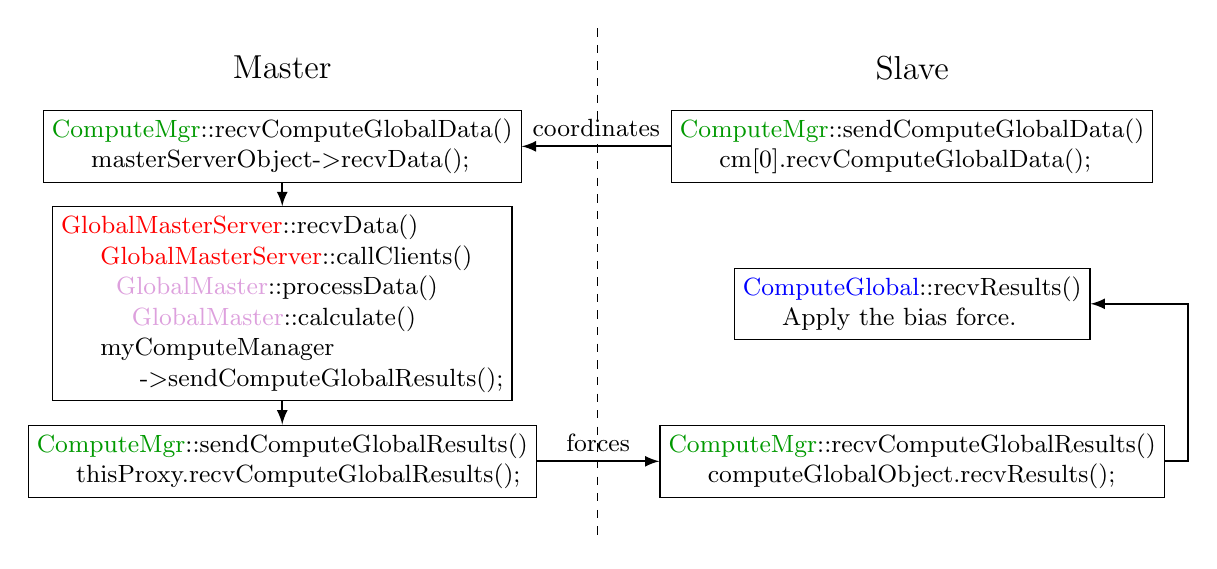
\begin{tikzpicture}\small

    \node[] (master) at (0, 10) {\large Master};

    \draw[dashed] (4, 10.5) -- (4, 4);

    \node[draw, align=left] (masterRecv) at (0, 9)
    { \textcolor{dkgreen}{ComputeMgr}::recvComputeGlobalData() \\
      \hskip 5mm masterServerObject-\textgreater recvData(); };

    \node[draw, align=left] (GlobalMasterServer) at (0, 7)
      { \textcolor{red}{GlobalMasterServer}::recvData() \\
      \hskip 5mm  \textcolor{red}{GlobalMasterServer}::callClients() \\
      \hskip 7mm \textcolor{Plum}{GlobalMaster}::processData() \\
      \hskip 9mm \textcolor{Plum}{GlobalMaster}::calculate() \\
      \hskip 5mm myComputeManager \\
      \hskip 10mm -\textgreater sendComputeGlobalResults(); };


    \node[draw, align=left] (masterSend) at (0, 5)
    { \textcolor{dkgreen}{ComputeMgr}::sendComputeGlobalResults() \\
      \hskip 5mm thisProxy.recvComputeGlobalResults(); };

    \node[] (slave) at (8, 10) {\large Slave};

    \node[draw, align=left] (slaveSend) at (8, 9)
    { \textcolor{dkgreen}{ComputeMgr}::sendComputeGlobalData() \\
      \hskip 5mm cm[0].recvComputeGlobalData(); };

    \node[draw, align=left] (slaveRecv2) at (8, 7)
      { \textcolor{blue}{ComputeGlobal}::recvResults() \\
      \hskip 5mm Apply the bias force. };

    \node[draw, align=left] (slaveRecv) at (8, 5)
    { \textcolor{dkgreen}{ComputeMgr}::recvComputeGlobalResults() \\
      \hskip 5mm computeGlobalObject.recvResults(); };

    \draw[->, >=latex, thick]
      (masterRecv) edge (GlobalMasterServer)
      (GlobalMasterServer) edge (masterSend);

    \draw[->, >=latex, thick]
      (slaveSend) edge node[anchor=south]{coordinates} (masterRecv);

    \draw[->, >=latex, thick]
      (masterSend) edge node[anchor=south]{forces} (slaveRecv);

    \draw[->, >=latex, thick]
    (slaveRecv) -| (11.5,6) |- (slaveRecv2);
  \end{tikzpicture}
\end{figure}

\subsection{ComputeMgr}

The code \texttt{ComputeMgr}
gives the structure of master/slave set-up.
%
\begin{lstlisting}
// this function is called in Node::startup() phase 10
void ComputeMgr::createComputes(ComputeMap *map) {
  Node *node = Node::Object();
  SimParameters *simParams = node->simParameters;

  if ( simParams->globalForcesOn && node->myid == 0 ) {
    /* create a master server to allow multiple masters */
    masterServerObject = new GlobalMasterServer(this,
            PatchMap::Object()->numNodesWithPatches());
    /* create the individual global masters */
    if (simParams->tclForcesOn) // adding to ->clientList
        masterServerObject->addClient(new GlobalMasterTcl());
    ...
  }
}

// slave call this function to send the master coordinates
void ComputeMgr::sendComputeGlobalData(ComputeGlobalDataMsg *msg) {
  CProxy_ComputeMgr cm(CkpvAccess(BOCclass_group).computeMgr);
  cm[0].recvComputeGlobalData(msg);
}

// master calls this via charm++, to receive coordinates
void ComputeMgr::recvComputeGlobalData(ComputeGlobalDataMsg *msg) {
  masterServerObject->recvData(msg);
}

// master calls this in GlobalMasterServer::callClients()
// to send slaves the global forces
void ComputeMgr::sendComputeGlobalResults(ComputeGlobalResultsMsg *msg) {
  msg->seq = ++computeGlobalResultsMsgMasterSeq;
  thisProxy.recvComputeGlobalResults(msg);
}

// slave calls this via charm++ to receive the global forces
void ComputeMgr::recvComputeGlobalResults(ComputeGlobalResultsMsg *msg) {
  if ( computeGlobalObject && msg->seq == computeGlobalResultsMsgSeq ) {
    CmiEnableUrgentSend(1);
    computeGlobalObject->recvResults(msg);
    CmiEnableUrgentSend(0);
  }
}
\end{lstlisting}


\subsection{ComputeGlobal}

Slave-end code.
%The class \texttt{ComputeGlobal} inherits \texttt{ComputeHomePatches}.

\begin{lstlisting}
// called when a slave receives the global force
// called by ComputeMgr::recvComputeGlobalResults()
void ComputeGlobal::recvResults(ComputeGlobalResultsMsg *msg) {
  // set the forces only if we aren't going to resend the data
  if( !msg->resendCoordinates ) { // apply forces to patches
    AtomMap *atomMap = AtomMap::Object();
    ResizeArrayIter<PatchElem> ap(patchList);

    for (ap = ap.begin(); ap != ap.end(); ap++) {
      (*ap).r = (*ap).forceBox->open();
      forcePtrs[(*ap).patchID] = (*ap).r->f[Results::normal];
      atomPtrs[(*ap).patchID] = (*ap).p->getAtomList().begin();
    }

    AtomIDList::iterator a = msg->aid.begin();
    ForceList::iterator f2 = msg->f.begin();
    for ( ; a != msg->aid.end(); ++a, ++f2 ) {
      LocalID localID = atomMap->localID(*a);
      if ( localID.pid == notUsed || ! forcePtrs[localID.pid] ) continue;
      forcePtrs[localID.pid][localID.index] += *f2;
      FullAtom &atom = atomPtrs[localID.pid][localID.index];
    }
  }
}

void ComputeGlobal::sendData() {
  // Get positions from patches
  AtomMap *atomMap = AtomMap::Object();
  const Lattice & lattice = patchList[0].p->lattice;
  ResizeArrayIter<PatchElem> ap(patchList);
  ComputeGlobalDataMsg *msg = new  ComputeGlobalDataMsg;

  msg->step = patchList[0].p->flags.step;
  for ( AtomIDList::iterator a = aid.begin(); a != aid.end(); ++a ) {
    LocalID localID = atomMap->localID(*a);
    if ( localID.pid == notUsed || ! atomPtrs[localID.pid] ) continue;
    msg->aid.add(*a);
    FullAtom &atom = atomPtrs[localID.pid][localID.index];
    msg->p.add(lattice.reverse_transform(atom.position, atom.transform));
  }

  comm->sendComputeGlobalData(msg);
  comm->enableComputeGlobalResults();
}
\end{lstlisting}




\subsection{GlobalMasterServer}


Master-end code (framework).

\begin{lstlisting}
// called at the beginning of simulation in ComputeMsg::createComputes()
// a client is a specialized master, e.g., GlobalMasterTcl
void GlobalMasterServer::addClient(GlobalMaster *newClient) {
  clientList.add(newClient);
  newClient->setLattice(&lattice);
}

// handle coordinates from slaves,
// called by ComputeMgr::recvComputeGlobalData()
void GlobalMasterServer::recvData(ComputeGlobalDataMsg *msg) {
  // handle msg ...
  if(recvCount == numDataSenders + numForceSenders + 1) {
    ...
    int resendCoordinates = callClients();
  }
}

int GlobalMasterServer::callClients() {
  for ( GlobalMaster **m_i = clientList.begin();
        m_i != clientList.end(); m_i++ ) {
    GlobalMaster *master = *m_i;
    master->processData(...);
  }
  ...
  ComputeGlobalResultsMsg *msg = new ComputeGlobalResultsMsg;
  ...
  // expanding the function resetForceList(msg->aid,msg->f,...);
  // iterate over all of the masters
  // e.g., (*m_i) may be a point to GlobalMasterTcl
  for ( GlobalMaster **m_i = clientList.begin();
        m_i != clientList.end(); m_i++ ) {
    /* add all of the atoms in this master */
    for(int i = 0; i < (*m_i)->forcedAtoms().size(); i++) {
      msg->aid.add((*m_i)->forcedAtoms()[i]);
      msg->f.add((*m_i)->appliedForces()[i]);
      ...
    }
  }
  myComputeManager->sendComputeGlobalResults(msg);
  return 0;
}
\end{lstlisting}


\subsection{GlobalMaster}

Here is the interface of the master end.
\begin{lstlisting}
class GlobalMaster {
  // after receiving the coordinates, things to do before
  // sending out the global force
  // calls the virtual function calculate();
  void processData(...);

  // basically, all we need to do is to
  // inherit GlobalMaster, and override this method
  virtual void calculate();

  AtomIDList &modifyForcedAtoms(); // returns fAtoms
  ForceList &modifyAppliedForces(); // returns appForces

  bool appForcesChanged;
  AtomIDList fAtoms; // atoms that are being forced
  ForceList appForces; // the corresponding forces
};
\end{lstlisting}


\section{HomePatch}

This is a patch of atoms that are handled by a computing node.


\section{Misc.}

The seed of the random number generator is initialized in SimParameters.C
Search the variable \texttt{randomSeed}.

The initial velocities is initialized in WorkDistrib.C,
\texttt{createHomePatches() --> createAtomLists() --> random\_velocities()}
before Sequencers are created.

But these random velocities are subject to rattle in Sequencer::integrate().

Another way to reinitialize velocities in to use the function
\texttt{reinitVelocities()} in Sequencer.C.
This is only invoked if there is a command 
\texttt{reinitvels 300} in the configuration file.




%\bibliographystyle{plain}
%\bibliography{simul}
\end{document}
